\documentclass[conference]{IEEEtran}
\usepackage{cite}
\usepackage[pdftex]{graphicx}
  \graphicspath{{img/}}
  \DeclareGraphicsExtensions{.png,.jpg}
\usepackage{fixltx2e}
\usepackage{url}


\begin{document}


\title{Crypton: Zero-Knowledge Application Framework}

\author{
  \IEEEauthorblockN{David Dahl}
  \IEEEauthorblockA{Project Director\\ ddahl@spideroak.com}
  \and
  \IEEEauthorblockN{Cam Pedersen}
  \IEEEauthorblockA{Principal Engineer\\ cam@spideroak.com}
}

\maketitle

\begin{abstract}
INCOMPLETE DRAFT DO NOT DISTRIBUTE

Applications intended to work on multiple devices or those that
store large enough amounts of data must save their data to a backend server
rather than locally. Privacy of users is typically only protected on the wire
with SSL or on the backend with an encrypted database. This leaves user data
and communications open to malicious server operators or attackers.
Application developers may easily fall into cryptographic
mistakes if they attempt to build on primitives themselves.

Crypton uses end-to-end encryption, provides application developers
with high-level APIs for user accounts, robust data storage, and
sharing information between users. We detail the framework's cryptographic
structure and its implementation architecture.
\end{abstract}

\section{Introduction}
Users' concern for the privacy of their data has become widespread
after numerous data leaks and revelations of widespread government spying\cite{spying}.
Applications built upon zero-knowledge principals have a competitive
advantage in an emulous market. Additionally, as a service operator,
it is inherently responsible to protect users' data from intrusions
by yourself or an adversary.

Crypton is a unique way to build applications, primarily because it
makes it simple for developers to store data with a server in such a way
that the server doesn't know what that data is.
Additionally, all Crypton-based applications are built solely on the client,
and the server acts as a smart pipe to the database to store and retrieve data
for authenticated users. A side effect of this architecture is that working with the framework is not dissimilar to using a "backend as a service".

Crypton's initial implementation has been built with JavaScript on the
client and server. JavaScript was chosen as it is the language of the web
and the large body of developers already engaged in JavaScript development.
JavaScript has also established itself in desktop and mobile rapid application
environments such as Microsoft Windows\cite{JavaScriptWindows},
Cordova\cite{Cordova} and node-webkit\cite{nodewebkit}.
This has led to several design considerations (which are...).
In this paper however, we will concentrate on the framework's
concepts moreso than its implementation details. These concepts may be used
to port the client side to nearly any platform.

\subsection{Motivation}
Moving forward from the success of SpiderOak's desktop backup client,
the logical progression is to use the Zero-Knowledge concepts in new ways,
specifically in communications applications popular on mobile devices
and desktop computers. Internet users today are tracked in unprecedented
ways by the advertising juggernaut that exists on the web as well as the
constant, blanket surveillance employed by many governments.
Email has always been about as private as sending a post card via the mail
service, while some headway has been made in making SSL/TLS the standard
way of protecting SMTP, there are glaring gaps. With this in mind,
SSL is not ever-present on all servers our browsers connect to,
and even if it was, there are massive problems with SSL and the
Certificate Authority system as a whole. A few of these issues are
Certificate Authorities being tricked into or via intrusion issuing
"valid" certificates that allow a man-in-the-middle attack to be almost
trivial to pull off, as well as massive zero-day bugs in popular SSL
encryption libraries such as OpenSSL.

The best defense includes the concept of 'defense-in-depth'\cite{defenseindepth}.
One technique is to use end-to-end encryption as well as an encrypted network
channel to move private data back and forth to servers and between users.
Making this easy for everyday developers who are not security experts is
paramount to its proliferation. This brings us to the User Experience (UX) of
cryptography in the realm of both developers and end users of Crypton-based
applications.

Crypton is primarily an exercise in improving the UX of cryptographic
software both from the software engineer's perspective and the
end users who use said software. Starting with the framework,
we employ JavaScript itself as an improvement in the UX of building
more private and secure applications. The Crypton tool set is well known
and loved by developers: node.js, Redis and PostgreSQL. The APIs that
Crypton provides are elegant and require no special knowledge of cryptographic
algorithms, methods, or mathematics. It is designed to be elegant, requiring,
for instance, a username, passphrase, and callback function in order to create
an account and generate the key ring. Below the surface, all cryptographic
operations are hidden.

\subsection{Zero Knowledge}
We define Zero Knowledge as a server's inability to access plaintext data while
maintaining its duties to store and secure that data. Crypton does not employ a
traditional zero-knowledge proof other than its use of the SRP\cite{SRP}
protocol for user authentication.

\subsection{Open Source}
A primary impetus behind turning this cryptosystem into a framework for
application developers is that a number of eyes on one project will find mistakes
faster than the same amount of eyes on many projects. Therefore,
making the codebase, development process, technical specification,
and issue tracker open source is a paramount motivation.

\subsection{Related Work}

\subsubsection{SJCL}
SJCL is a JavaScript library that implements a set of cryptographic 
primitives\cite{sjcl}. It is used in Crypton until a native bridge API
such as the Web Crypto API has found sufficient footing in browsers.
While SJCL was chosen over several other similar libraries, such as
CryptoJS\cite{cryptojs}, for speed and feature concerns,
it is still slower than a native option would allow. Additionally,
key material is hard to guard from exploits such as XSS in an interpreted
environment. We will revisit these concerns later in the paper.

\subsubsection{Mylar}
Mylar\cite{mylar} is a project with aspirations similar to
Crypton - encrypting and decrypting users' data in a browser context.
However, it also attemps\cite{mylarpaper} to solve extraneous problems
such as server-side keyword search over encrypted documents. We have chosen
to keep Crypton as simple as possible and allow developers to add functionality
like this by use of Crypton's client-side Container structures.

Mylar is intended to be used in the browser as a traditional web application,
employing a browser extension to verify dynamically loaded code. Crypton is meant
to exist in a packaged mobile or desktop application.

\subsubsection{End-to-End}
Google has created a Chrome extension\cite{endtoendblog} emulating a
PGP system in the browser using OpenPGP\cite{endtoend}. Unlike Crypton,
it does not seek to provide a framework for developing applications,
but to simplify the addition of end-to-end encryption in existing applications.
Like Mylar, it requires a browser extension to use.

Its key distribution relies on a web of trust\cite{endtoendkeydistribution},
whereas Crypton's relies on manual, out-of-band fingerprint verification.

\section{Architecture}

\subsection{Backend}
PostgreSQL was chosen for the main data store for its ACID compliance,
transaction handling, and replication options.

Redis was chosen as a session store for its speed.
Due to the nature of Crypton's composable transactions,
session-authenticated requests may hit the server quickly or en masse.

Node.js was chosen for an HTTP server and transaction processing logic.
Its event-driven architecture was desirable, as well as the reduced
context switching in development and possibility of isomorphic code
that language parity with the client brings.

Docker is used to homogenize backend deployment. This leads to ease of
use from a development perspective and the hope of decreased server
security mistakes that a unified process brings.

%\subsection{Ciphers}
%Before continuing, it is important to note that all future mentions
%of encryption or decryption assume AES256 in Gallois/Counter Mode %(GCM)\cite{gcm}.
%We utilize the Elgamal encryption scheme using elliptic curve p384 for keys.
%CLEAN ME UP! \^\

\subsection{Frontend}
Crypton clients may be implemented in any context where their code may be
packaged and verified. All data is passed RESTfully using JSON over SSL.

\subsection{Accounts}
Each user of a Crypton application must have an Account.

\subsubsection{Authentication}
Authentication is achieved without storing a password equivalent
(hash or otherwise) by use of the Secure Remote Password Protocol (SRP)
\cite{srp-protocol}. After a successful SRP negotiation, the client uses
the user's \(password\) and \(keypair\_salt\) to generate a \(keypair\_key\)
with PBKDF2\cite{pbkdf2}. A \(keypair\_mac\_key\) is also generated with
the \(keypair\_mac\_salt\).

The \(keypair\_key\) is used to decrypt the 

\subsubsection{Keyring}
Each account has a keyring.

\begin{table}[ht]
\caption{Crypton Keyring Storage Fields}
\centering
\begin{tabular}{l l}
\hline\hline
\\ [0.1ex]
Field & Purpose \\
\\ [0.1ex]
\hline
\\ [0.3ex]
srp\_verifier & SRP \(v\) (password verifier) \cite{srp-protocol} \\
srp\_salt & SRP \(s\) (user's salt) \cite{srp-protocol} \\
keypair\_salt & salt used to generate \(keypair\_key\) \\
keypair\_mac\_salt & salt used to generate \(keypair\_mac\_key\) \\
keypair & main keypair encrypted by \(keypair\_key\) \\
keypair\_mac & MAC used to verify \(keypair\) \\
pubkey & plaintext public key for account \\
container\_name\_hmac\_key & key used for HMAC of container names \\
hmac\_key & key used for generalized HMAC operations \\
sign\_key\_pub & plaintext public key for signature verification \\
sign\_key\_private\_mac\_salt & salt used to generate \(sign\_key\_private\_mac\) \\
sign\_key\_private & ciphertext of private signature key, \\
sign\_key\_private\_mac & MAC used to verify \(sign\_key\_private\) \\
\\ [0.3ex]
\hline
\end{tabular}
\label{table:nonlin}
\end{table}


\subsection{Transactions}
All client operations which affect the state of the database are performed
with composable transactions. These are typically hidden from developers -
clients abstract common transactions such as account and container creation
to provide a transparent API - however they can be used manually to create
new atomic action sets.

\subsubsection{Transaction Chunks}
Transaction Chunks are the actions which may be individually or collectively
added to a transaction. Data attached to a Chunk is referred to as its "payload".
It may require specific data or none at all.

\subsubsection{Transaction Lifecycle}
Transactions must first be created - this provides a unique identifier for
all future actions regarding that transaction. Transaction Chunks can be added
in batch or one at a time. Transactions must have one or more Chunks to be
considered valid.

When a client is done composing a transaction, it may request the backend
to commit it. This is typically a synchronous operation from the client's
perspective, but transaction processing is up to the backend's discretion.

\begin{table}[ht]
\caption{Crypton Transaction Chunk Types}
\centering
\begin{tabular}{l l}
\hline\hline
\\ [0.1ex]
Name & Purpose \\
\\ [0.1ex]
\hline
\\ [0.3ex]
add\_account & create an account \\
set\_base\_keyring & add or change keyring for account \\
add\_container & create a new container \\
delete\_container & delete an existing container \\
add\_container\_session\_key & add session key for container \\
add\_container\_session\_key\_share & add wrapped session key \\ & \ \ for a given container and account \\
add\_container\_record & add a new record for given container \\
add\_message & add a user-to-user message \\
delete\_message & delete a user-to-user message \\
\\ [0.3ex]
\hline
\end{tabular}
\label{table:nonlin}
\end{table}

\subsubsection{Transaction Processing}
As Chunks are added to a transaction, they are added as rows in
pre-processing tables in the database. When a client requests that the
transaction be committed, it is marked with a commit request time and added
to a queue.

A separate dequeueing program (or likely a clustered deployment of said program) 
will watch for and process incoming transactions. All pre-processing rows are
pulled from the database which belong to the transaction in question. This
data is checked for logical consistency (a record may not be added to a
nonexistant container) and stored in temporary tables. It is then checked for
semantic consistency (two accounts may not have the same username) and its
changes are commited to the database.

CLEAN ME UP \^

\subsection{Containers}
Containers provide the main logical abstraction for data storage in Crypton.
On the client, they are meant to resemble (or replicate) the interface of
the implementation language's native object format (an Object in JavaScript or
a Dictionary in Python). They are meant to be used as a native data structure,
with a few exceptions.

The first exception is that Containers have names. This name is only known to
the client; to interact with the container (through transactions),
the client must first HMAC the container name with their account's
\(container\_name\_hmac\_key\).

The second exception is that they may be saved. When they are saved, a
Container Record is created. MORE \^

\subsubsection{Container Records}
Container Records are defined as discrete changes between versions of a
container.

When a container is saved on a client, the delta between its
last known version is calculated and encrypted. This is sent the server
with the \(add\_container\_record\) transaction chunk.

When a container is loaded, all of its encrypted deltas are sent to the
client, are decrypted, and the state of the object is rebuilt using them.

\subsubsection{Container Session Keys}
Container Records are encrypted with a per-container key called the Container
Session Key.

\subsubsection{Container Session Key Shares}
Container Session Key Shares are wrapped versions of Container Session Key.
When a container is loaded, the server will send the client a 
\(container\_session\_key\_share\) for its account, which it must decrypt with
its private key, providing a \(container\_session\_key\).

This allows a container to be shared with another account by a user who
already has access to that container. This is done by encrypting the
\(container\_session\_key\) with that user's public key.
Giving oneself access to a container and sharing that container are effectively
the same operation.

\subsection{Messages}
Messages are an additional data structure Crypton provides for when Containers
are not the best option - typically in a situation where you have to send
data to another user in a one-off fashion and don't require versioning or
sharing.

Crypton Messages are implemented traditional public-key messages.

\subsubsection{Headers}

\subsection{Peers}
Each user account is considered a "Peer". A Peer's existence can be ascertained if the querying user knows the exact Peer username:

% TODO code styling??
session.getPeer('alice', function(err, peer) {});

Once a peer is known, a fingerprint verification is required in order to establish the peer in the user's trusted contacts container\cite{trustStateContainer}

A peer cannot be communicated with unless it exists inside the 'trustStateContainer'.

\subsubsection{Peer Verification}
Peer verification is best performed in an out-of-band manner. The best approach here is for an app developer enable the app to send an out of band email or sms message to relay the fingerprint of user "alice" to user "bob". Once the Bob has Alice's fingerprint, he can verify it against the peer.fingerprint stored on the Crypton server. With a match, Bob can "verify" Alice and her peer data (username, fingerprint, public key) can then be stored in Bob's "Trust State Container"\cite{trustStateContainer}

\subsection{Trust State Container}
The "Trust State Container" is a normal Crypton container that is generated during account generation. This conatiner is used to keeo track of each peer that a user verifies out of band via a fingerprint sent over SMS, email, or perhaps even collected vi a QRCode\cite{QRCode}.

These peer/fingerprint APIs and verification steps (especially if used in an "out of band" manner), allow for a system that can detect changed fingerprints on the server in order to warn users that the peer they want to communicate with might be an imposter.

\subsestion{New Metaphors}
Crypton's peer verification and contact storage mechanisms include an effort to create new metaphors in privacy-centered applications. Instead of using terms like "Fingerprint" and "Public Key", we want to find a metaphor that everyday Internet users better understand. Our most recent API includes an object called "Card". Card can generate an "ID Card" for each user that can be sent out of band as an SMS or email attachment. This ID card has a fingerprint on it, but also includes the username, a QRCode and an "Identigrid". The "Identigrid" is a 4X4 square color grid that translates the plain text fingerprint to colors, making it easier to quickly verify it.

Naturally, the use of a QRCode\cite{QRCode} allows developers to nearly automate the fingerprint verification and key exchange. We strongly encourage developers to use the QRCode as it allows for more automation. The Crypton team has planned for some UX research in 2015 around the "Identigrid" concept versus manual fingerprint verification of long strings.

% Add Identigrid Image here
\begin{figure}[h]
  \centering
  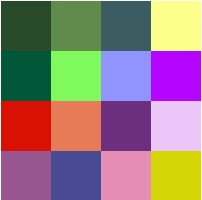
\includegraphics[width=0.3\textwidth]{identigrid-example.jpg}
  \caption{Identigrid}
\end{figure}

% Add ID CARD Image here
\begin{figure}[h]
  \centering
  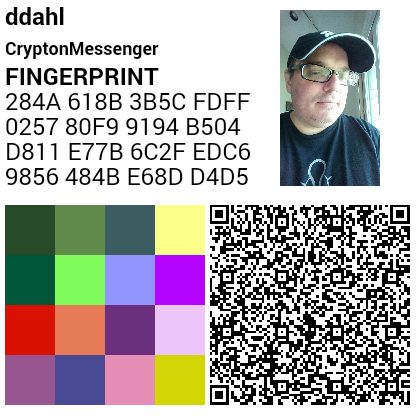
\includegraphics[width=0.3\textwidth]{id-card-example.png}
  \caption{ID Card with Photo}
\end{figure}

The basic concept is that Bob needs a copy of Alice's ID Card and Alice needs a copy of Bob's in order to establish a private communications channel. With the plain text fingerprint, "Identigrid", QRCode (and perhaps a photo), the verification of a peer becomes a familiar step to the vast majority of users who understand what an ID card in the physical realm is. 

{Threat Model}
\subsection{Assumptions}
Crypton has initially been developed in JavaScript, however, there are no
apparent difficulties in porting these concepts to a another language.
In its use of JavaScript, it could be easily assumed that Crypton was meant to
be used in a web browser - this is incorrect. Browsers are beset by a problem of
unverifiable code delivery in that users cannot verify that
the code they received is as intended. Therefore, it is only recommended to use
Crypton in packaged applications. Tools such as Cordova or node-webkit are
recommended for packaging Crypton-based applications.

\subsection{Guarantees}

\subsection{Threats}

\subsubsection{IP storage}
\subsubsection{Peer graph analysis}
\subsubsection{Container access frequency analysis}

\subsection{Key Distribution}

\section{Performance}

\section{Additional Considerations}

\subsection{Federation}
\subsection{Advertisement}

\section{Use Cases}
This section could grow too large. Let's get rid of it?

\subsection{Private Diary}
\subsection{Encrypted Search}
\subsection{Private Location Sharing}

\section{Future Work}

\subsection{Container Compaction}
\subsection{Multiple Client Implementations}
\subsection{Hosted Backend}
\subsection{Zero Knowledge Payments}

\section{Conclusion}
The conclusion goes here.

\section{Call To Action}
Modern application developers have the \footnote{regrettably} new found responsibility
to protect their users' data.

Whether you utilize Crypton or not, the authors implore you to protect yourself
and your users from adversaries by encrypting all data, not only on the wire but at rest.

\section*{Acknowledgment}
The authors would like to thank...

\newpage
\begin{thebibliography}{20}
\bibitem{JavaScriptWindows} \url{http://msdn.microsoft.com/en-us/library/windows/apps/br229565.aspx}
\bibitem{Cordova} \url{http://cordova.apache.org/}
\bibitem{nodewebkit} \url{https://github.com/rogerwang/node-webkit}
\bibitem{defenseindepth} \url{http://en.wikipedia.org/wiki/Defense_in_depth_%28computing%29}
\bibitem{spying} \url{https://www.eff.org/nsa-spying}
\bibitem{SRP} \url{https://www.ietf.org/rfc/rfc2945.txt}
\bibitem{sjcl} \url{https://crypto.stanford.edu/sjcl/}
\bibitem{webcrypto} \url{http://www.w3.org/TR/WebCryptoAPI/}
\bibitem{cryptojs} \url{https://code.google.com/p/crypto-js/}
\bibitem{xss} \url{https://en.wikipedia.org/wiki/Cross-site_scripting}
\bibitem{mylar} \url{http://css.csail.mit.edu/mylar/}
\bibitem{mylarpaper} \url{http://css.csail.mit.edu/mylar/mylar.pdf}
\bibitem{endtoend} \url{https://code.google.com/p/end-to-end/}
\bibitem{QRCode} \url{http://www.qrcode.com/en/about/}
\bibitem{endtoendkeydistribution} \url{https://code.google.com/p/end-to-end/wiki/KeyDistribution}
\bibitem{endtoendblog} \url{http://googleonlinesecurity.blogspot.com/2014/06/making-end-to-end-encryption-easier-to.html}
\bibitem{srp-protocol} \url{http://srp.stanford.edu/design.html}
\bibitem{pbkdf2} \url{https://tools.ietf.org/html/rfc2898}
\bibitem{gcm} \url{http://csrc.nist.gov/publications/nistpubs/800-38D/SP-800-38D.pdf}
\bibitem{IEEEhowto:kopka} H.~Kopka and P.~W. Daly, \emph{A Guide to \LaTeX}, 3rd~ed.\hskip 1em plus 0.5em minus 0.4em\relax Harlow, England: Addison-Wesley, 1999.
\bibitem{trustStateContainer} A default Crypton container that holds all "trusted" contact usernames and  public key fingerprints
\end{thebibliography}
\end{document}
